\section{The Rest of Probabilistic Evaluation: Optimization and
  Evaluation}
\label{passert:sec:mechanisms}

To verify a conditional in a \passert, probabilistic evaluation
extracts a symbolic representation of the conditional, optimizes this
representation, and evaluates the conditional.  The previous sections
described the distribution extraction step and this section describes our
optimization and evaluation steps. 

Optimizations simplify the Bayesian network by applying known
statistical properties to make verification more efficient. In
restricted cases, these optimizations simplify the Bayesian network to a
closed-form Bernoulli representing the condition in the \passert and we thus
evaluate the \passert exactly. In the general case, we use sampling
and hypothesis testing to verify it statistically.

\subsection{Optimizing Bayesian Networks}
\label{passert:sec:optim}

This section enumerates the statistical
properties that \tool applies to simplify distributions.

\paragraph{Closed-Form Operations on Known Distributions}
\tool exploits closed-form algebraic operations on the common
Gaussian, uniform, and Bernoulli distributions.
For example, if $X \sim N(\mu_x, \sigma^2_x)$ and $Y \sim N(\mu_y,
\sigma^2_y)$ then $X + Y \sim N(\mu_x + \mu_y, \sigma^2_x +
\sigma^2_y)$.  Likewise, if $X \sim N(\mu_x, \sigma^2_x)$ then $X + 3
\sim N(\mu_x + 3, \sigma^2_x)$.  \tool optimizes closed form addition
of Gaussians and scalar shifts or scaling of Gaussians, uniforms, and
Bernoullis.  We note there are many distributions and operations which
we do not yet encode (e.g., a sum of uniform distributions is
an Irwin--Hall distribution).
Expanding the framework to capture a larger catalog of statistical properties is left
to future work.

\paragraph{Inequalities Over Known Distributions} \tool uses the
cumulative distribution function (CDF) for known distributions to
simplify inequalities.  The CDF for a real-valued random variable $X$ is
the function $F_X$ such that $F_X(x) = \prob{X < x}$, which provides a
closed-form mechanism to evaluate whether a distribution is less than
a constant.  For example, if $X \sim U(0,1)$ and the programmer writes
the inequality $X < 0.9$, we reduce the inequality
to a Bernoulli because $F_{\mathit{Uniform}}(0.9) = \prob{X < 0.9} = 0.9$.  

\paragraph{Central Limit Theorem} The sum of a large number of
independent random variables with
finite variance tends to a Gaussian.  \tool uses the Central Limit
Theorem to reduce loops which compute a reduction over random
variables into a closed-form Gaussian which samples from the body of
the loop.  This transformation resembles the mean pattern exploited by
Misailovic et al.~\cite{sasa-sas}. It is particularly
effective on the 
\bench{sobel} application used in our evaluation, which averages the errors for each pixel in an
array. \tool reduces this accumulation to a single Gaussian.

\paragraph{Expectation Propagation}
\label{passert:sec:expectation}

The prior optimizations all approximately preserve a program's semantics: 
the transformed Bayesian network is approximately equivalent to the original
Bayesian network.
However, using statistical laws that apply to inequalities over random
variables, it suffices to instead compute only the expected value and variance
of a distribution.
\tool uses this insight to
further simplify Bayesian networks by exploiting (1) the linearity of
expected value and (2) statistical properties of inequality.

First, \tool uses the linearity of expectation to produce simpler
distributions with the same expected value as the original
distribution. This is an important optimization because verifying a \passert
amounts to calculating the expected value of its underlying Bernoulli
distribution. 
For example, the Bayesian network for
$D + D$, which computes two independent samples from $D$,
is not equivalent to the Bayesian network induced from $2 \cdot
D$. So an optimization resembling traditional strength reduction does
not compute the correct distribution.
However, these two Bayesian networks have the same expected
value. Specifically, expectation has the property $\expc{A + B} =
\expc{A} + \expc{B}$ for all distributions $A$ and $B$.
When only the expected value is needed, \tool optimizes $D + D$ to $2 \cdot
D$.
A similar property holds for variance when the random variables are
uncorrelated.

The reasoning extends to comparisons via Chebyshev's inequality.
Given the expectation $\mu$ and variance $\sigma^2$ of a random variable,
Chebyshev's inequality
gives a bound on the probability that a sample of a random variable deviates
by a given number of standard deviations from its expected value.
For example, for a program with
\lstinline{passert x >= 5}, distribution extraction produces a Bayesian
network of the form $X \ge 5$.
Using the linearity of expectation, say we statically compute that $\sigma = 3$ and $\mu = 1$ for
$X$. Chebyshev's inequality states:
%
$$\prob{|X - \mu| \ge k\sigma} \le \frac{1}{k^2}$$
%
We want to bound the probability that $x \ge 5$. Since we have $\mu$ and $\sigma$, we can rewrite this condition as:
%
\begin{align*}
x &\ge \mu + 2\sigma \\
x - \mu &\ge 2\sigma
\end{align*}
%
So the \passert condition states that $x$ deviates from its mean by at least 2
standard deviations. Using $k=2$ in Chebyshev's inequality gives the bound:
%
$$\prob{X \ge 5} \le \frac{1}{2^2}$$
%
We now have a bound on the probability (and hence the expectation) of the
inequality \code{x >= 5}.


\subsection{Verification}
\label{passert:sec:verification}
This section describes how we use a simplified Bayesian network to verify
\passerts using (1) exact (direct) evaluation or (2) sampling and
statistical hypothesis testing.

\subsubsection{Direct Evaluation}
\label{passert:sec:exact}
In some cases, simplifications on the probability distribution are
sufficient to fully evaluate a \passert. For example, \tool simplifies
the \bench{sobel} application in our evaluation to produce a
distribution of the form $\sum_n D < c$. The Central Limit Theorem
optimization replaces the sum with a Gaussian distribution, which then
enables the inequality computation to produce a simple Bernoulli
distribution with a known probability.  When dealing with a single
Bernoulli, no sampling is necessary. \tool reports the probability
from the simplified distribution.

\subsubsection{Statistical Verification via Sampling}
\label{passert:sec:sample}

In the general case, optimizations do not completely collapse a probability
distribution. Instead, \tool samples the resulting distribution to estimate its
probability.

\tool uses acceptance sampling to bound any error in its
verification~\cite{Younes}.  All \passert statements are logical
properties over random variables and therefore Bernoulli random
variables. Assume $X_i \sim \mathrm{Bernoulli}(p)$ is an independent sample of
a \passert where $p$ is the \emph{true} probability of the \passert,
the value \tool is estimating.
%
Let $X = X_1 + X_2 + \dots + X_n$ be the sum of $n$ independent
samples of the \passert and let the empirical expected value,
$\expc{X} = \overline{X} = X/n$, be an estimate of $p$.\footnote{This
  section uses $\overline{X}$ instead of \expc{X} for notational
  convenience.}  To bound error in its estimate, \tool computes
$\prob{\overline{X} \in \left[p - \epsilon, p + \epsilon\right]} \ge 1 - \alpha$.
In words, it tests whether there is at most an $\alpha$ chance that \tool's
estimate of $p$ is wrong. Otherwise, \tool's estimate of $p$ is within
$\epsilon$ of the truth.  A programmer can control the likelihood of a
good estimate---or the \emph{confidence}---by decreasing $\alpha$.
Likewise, a programmer can control the \emph{accuracy} of the estimate
by decreasing $\epsilon$. Because \tool uses sampling, it provides
statistical guarantees by testing whether its confidence
interval for $\overline{X}$ includes $p \pm
\epsilon$.  In concert, these parameters let a programmer trade off
false-positives and false-negatives with sample size.

In particular, given $\alpha$ and $\epsilon$, \tool uses the two-sided
Chernoff bound to compute $n$, the minimum number of samples required
to satisfy a given level of confidence and
accuracy~\cite{chernoff1952measure}. The two-sided Chernoff bound is
an upper-bound on the probability that an estimate, $\overline{X}$,
deviates from its true mean, $p$:
%
$$\prob{|\overline{X} - p| \ge \epsilon p} \le 2 e^{-\frac{\epsilon^2}{2 + \epsilon} np}$$
%
The left-hand side of the equality is $\alpha$ by definition and the worst
case (the most samples required) occurs when $p = 1$. Solving for $n$ yields:
%
$$n \ge \frac{2+\epsilon}{\epsilon^2}\ln\frac{2}{\alpha}$$
%
For example, at a confidence 95\% and an accuracy of 3\%:
%
$$n \ge \frac{2+0.03}{0.03^2}\ln\frac{2}{0.05}$$
%
meaning that \tool needs to take at least $n=8321$ samples.  Note that this bound
is an over-approximation of the true number of samples required for a
given level of confidence and accuracy---it only relies on $\alpha$
and $\epsilon$ and ignores how good an estimate $\overline{X}$ is of $p$.
An extension, which we leave to future work, is to use Wald's
\emph{sequential sampling} to iteratively compute $\prob{\overline{X}
    \in [p - \epsilon, p + \epsilon]} \ge 1 - \alpha$ after each
sample~\cite{wald1945sequential}. Because this approach uses the
current estimate of $\overline{X}$ relative to $p$, it is often able to
stop sampling well before reaching our
upper bound~\cite{Younes20061368}.

\paragraph{Statistical Guarantees}

The prior section describes how \tool turns a \passert statement into
a hypothesis test in order to
bound error in its estimate. If the property is sufficiently likely
to hold, \tool verifies the \passert as true.  Likewise, if the \passert is
verified as false,
the programmer needs to iterate, either by changing
the program to meet the desired specification or by correctly expressing the
probabilistic property of the program.

% To use that estimate, we note that if
% $\bar{X} + \epsilon \le 0.5$ then the \passert is \code{true} at the
% $\alpha$ confidence interval (i.e., it is more likely than not to be
% true).  Likewise, if $\bar{X} - \epsilon \ge 0.5$ the \passert is
% \code{false}. %  In those cases where $\bar{X}$ is indistinguishable
% from 0.5 are unable to verify this probabilistic assertion and thus
% return "unknown". As we demonstrate in Section~\ref{passert:sec:evaluation},
% with sufficient confidence and accuracy, unknown occurs infrequently
% in practice.
\begin{figure}
    \begin{centering}
    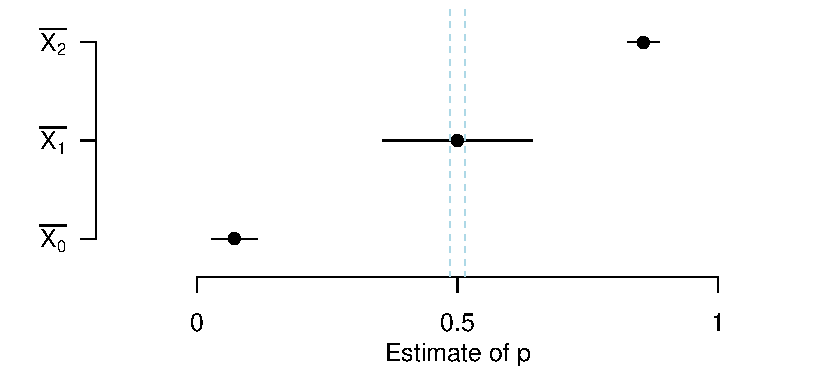
\includegraphics[width=\columnwidth]{figs/verification}
    \end{centering}
    \caption{Hypothesis tests for three different \passert statements.}
    \label{passert:fig:verify}
\end{figure}
For example, suppose \tool estimates $\prob{\overline{X}_i \in \left[p - \epsilon,
p + \epsilon\right]} \ge 1 - \alpha$ for three distinct, hypothetical \passert statements
(i.e., $i \in [0,1,2]$). We pictorially show these three estimates in
Figure~\ref{passert:fig:verify}. Each estimate shows $\overline{X}_i$ as a point
and lines depict the confidence region of that estimate.  
Because the confidence region of $\overline{X}_0$ is below $0.5$, \tool verifies
this assertion as false (i.e., the \passert rarely holds).  
Likewise, because $\overline{X}_2 - \epsilon \ge 0.5$, \tool verifies this
assertion as true (i.e., the \passert often holds).

However, at this confidence level and accuracy, \tool is unable to
verify $\overline{X}_1$ as its confidence region and thus estimate \emph{overlaps} with $0.5 \pm \epsilon$.  Thus, \tool
labels this assertion as unverifiable.  To verify this assertion as
true or false, the programmer must increase either the
confidence or accuracy (or both).  In this situation, \tool initiates
a dialog with the programmer for guidance on how to proceed.
